\documentclass{article}
\usepackage[utf8]{inputenc}
\usepackage{graphicx}
\usepackage{subfiles}
\usepackage{natbib}
\usepackage{gensymb}
\usepackage{hyperref}
\usepackage{geometry}
\geometry{
 a4paper,
 total={170mm,257mm},
 left=30mm,
 right=30mm,
 top=30mm,
 bottom=30mm,
}
\usepackage{lineno}
\linespread{2}

\title{The robustness of a simple dynamic model of island biodiversity to geological and sea-level change}
\author{Pedro Santos Neves*\textsuperscript{1}, Joshua W. Lambert*\textsuperscript{1}, Luis Valente\textsuperscript{1,2} and Rampal S. Etienne\textsuperscript{1}}
\date{}

\linenumbers

\begin{document}

\maketitle

\noindent $^{1}$ Groningen Institute for Evolutionary Life Sciences, University of
Groningen, Box 11103, 9700 CC Groningen, The Netherlands

\noindent $^{2}$ Naturalis Biodiversity Center, Darwinweg 2, 2333 CR Leiden, The Netherlands 

\noindent * These authors contributed equally to this work.

\noindent Corresponding Author: Pedro Santos Neves, Groningen Institute for Evolutionary Life Sciences, Box 11103, 9700 CC Groningen, The Netherlands. Email: p.m.santos.neves@rug.nl.

\section*{Abstract}

Aim: Biodiversity on islands is influenced by various geophysical processes and sea-level fluctuations. Oceanic islands (never connected to a landmass) are initially vacant with diversity accumulating via colonisation and speciation, followed by a decline as islands shrink. Continental islands have species upon formation (when disconnected from the mainland) and may have transient land-bridge connections. Theoretical predictions for the effects of these geophysical processes on rates of colonisation, speciation and extinction have been proposed. However, paleogeographic reconstructions are difficult to obtain and are currently unavailable for most islands, and methods of phylogenetic inference assume only oceanic island scenarios without accounting for island ontogeny, sea-level changes or past landmass connections. Here, we analyse to what extent ignoring geodynamics in the inference model affects model predictions when confronted with data simulated under a geodynamic model. \\

\noindent Location: Simulation of oceanic and continental islands. \\

\noindent Methods: We extend the island biogeography simulation model DAISIE to include area-dependent rates of colonisation and diversification associated with island ontogeny and sea-level fluctuations, and continental islands with biota present upon separation from the mainland, and shifts in colonisation to mimic temporary land-bridges. We quantify the error made when geodynamic processes are not accounted for by applying DAISIE’s inference method to geodynamic simulations. \\

\noindent Results: We find that the robustness of the model to dynamic island area is generally high (error is small) for oceanic islands and for continental islands that have been separated for a long time, suggesting that, for these island types, it is possible to obtain reliable results when ignoring geodynamics. However, for continental islands that have been recently or frequently connected, robustness of the model is low. \\

\noindent Main conclusions: This study highlights that under a large proportion of island biogeographic geodynamic scenarios (oceanic islands and ancient continental fragments) a simple phylogenetic model ignoring geodynamics is empirically applicable and informative. However, recent connection to the continent cannot be ignored, requiring development of a new inference model. Importantly, our results show that for oceanic islands, which have been crucial systems for the development of biogeographical theory, reliable insights can be obtained from phylogenetic data in the absence of paleogeographic reconstructions of island area. \\

\noindent \textbf{Keywords}: Community Assembly, Continental Island, DAISIE, Diversification, Island Biogeography, Island Ontogeny, Phylogenetic Analysis, Robustness Analysis \\

\clearpage

\noindent \textbf{Significance Statement}: Island biogeographic studies seek to understand how island communities assemble and diversify. While islands undergo geological and sea-level changes that affect biodiversity, data on geodynamic processes on islands is often lacking, and current phylogenetic models in island biogeography do not incorporate geological evolution. This study shows that despite not including geodynamics, a simple phylogenetic model (DAISIE) often accurately infers the history of biodiversity on islands subject to island ontogeny, sea-level changes and continental islands that have been isolated for a long period. However, the model is not robust to recently formed continental and land-bridge islands, elucidating the need for new phylogenetic methods for these island types. \\

\noindent \textbf{Biosketch}: The authors, based at the University of Groningen and Naturalis Biodiversity Center, develop and apply novel computational methods in island biogeography. They utilise community phylogenetic data to understand processes and patterns on islands over macroevolutionary timescales. \\

\noindent \textbf{Author contributions}: P.N., J.W.L., L.V., and R.S.E. conceived the ideas and methodology and wrote the code, P.N. and J.W.L. analysed the data and led the writing. L.V. and R.S.E. commented on the analysis and the manuscript.\\

\clearpage

\section*{Introduction}

The study of biodiversity on islands rests upon the foundational work of MacArthur and Wilson’s (\citeyear{macarthur_equilibrium_1963, macarthur_theory_1967}) equilibrium theory of biodiversity (ETIB). The theory describes island diversity as determined by species colonisation and extinction, governed by island area and isolation. The ETIB proposes that an equilibrium state of biodiversity emerges when the rates of colonisation and extinction are equal. Additionally, diversity can accumulate through \textit{in situ} speciation, particularly on large isolated islands \citep{macarthur_theory_1967, losos_analysis_2000, rosindell_unified_2011, valente_simple_2020}. While the ETIB has found empirical support at both ecological \citep{simberloff_experimental_1970} and evolutionary \citep{valente_equilibrium_2017, valente_simple_2020} time scales and while its fundamental mechanisms are generally accepted, the state of equilibrium is thought to not be easily reached or maintained \citep{heaney_dynamic_2000, whittaker_general_2008, valente_effects_2014, warren_islands_2015, fernandezpalacios_towards_2016, marshall_uncertain_2016}, because of frequent ecological, geological and sea-level perturbations. The general dynamic model (GDM), glacial sensitive model (GSM), and sea-level sensitive model (SLS) of island biogeography extend the ETIB by incorporating the influence of geodynamics (island ontogeny and sea-level) on evolutionary processes \citep{whittaker_general_2008, fernandezpalacios_towards_2016, avila_towards_2019}. Simulating these models has revealed empirical support for an effect of geodynamics on biodiversity \citep{whittaker_general_2008, bunnefeld_island_2012, steinbauer_re-evaluating_2013, rijsdijk_quantifying_2014, lim_true_2017}. \\

The trajectory of island diversity is a result of ecological and geological evolution. Among the relevant physical and biological island characteristics that influence island diversity, area stands out \citep{ali_islands_2017}. Islands are classified as oceanic or continental, differentiated by the latter having had a physical connection to a mainland at some point in their history \citep{wallace_island_1880, ali_islands_2018}. Continental islands form via a separation from a continental landmass and are stable or undergo a very slow decline in island area \citep{ali_islands_2018}. Here we use these broad terms but acknowledge the pronounced geological differences between and within various island types (see \cite{ali_islands_2017, ali_islands_2018}). Island ontogeny encapsulates the geological evolution of area, topographic complexity, and elevation over an island’s lifespan, which impact species diversity. Oceanic islands generally undergo an ontogeny that starts with initial island emergence, an uplift phase of rapid increase in area, until the island reaches a maximum size. This is followed by a relatively slow decline in area, and eventually atoll formation and submergence \citep{ramalho_coastal_2013, ali_islands_2017}. Oceanic island ontogeny is hypothesised to affect diversity. For example, the GDM uses a niche-based argument for a time-variable carrying capacity that governs speciation, extinction and colonisation as area changes \citep{whittaker_general_2008}. Simulations of the effects of island ontogeny on phylogenetic data show that island ontogeny can indeed influence species richness, but its effect depends on specific characteristics of the island in question \citep{valente_effects_2014}. Long-term area change through time due to island ontogeny is not the only factor to influence island diversity and to vary throughout the island’s lifespan. At shorter time scales, sea-level fluctuations also affect island area, as well as potentially altering island connectivity within an archipelago or with the mainland, by varying the distance between landmasses, for example through the formation of temporary land-bridges \citep{ali_exploring_2014, fernandezpalacios_towards_2016, hammoud_past_2021}. Dynamic island connectivity has left signatures on contemporary total and endemic island species diversity \citep{weigelt_late_2016, norder_beyond_2019}. However, it is possible that rapid fluctuations change short-term colonisation patterns without leaving a pronounced signature on phylogenetic and species richness data, effectively functioning as constant dynamics when observed over macroevolutionary timescales ($>$ 1 million years). \\

Most generalities of island biogeography derive from oceanic islands \citep{whittaker_general_2008}, limiting our understanding of continental islands, which, in fact, make up the vast majority of islands \citep{meiri_oceanic_2017}. Oceanic islands initially completely lack species, followed by diversity increasing through colonisation of mainland species. They tend to have a high proportion of endemics, given that many species undergo cladogenesis or anagenesis facilitated by island isolation \citep{valente_simple_2020}. Cladogenesis on oceanic islands of sufficient area has led to spectacular radiations \citep{losos_adaptation_2009}. Continental island biota have distinct evolutionary characteristics. Often, a proportion of their species have vicariant origins, deriving from the mainland pool upon island formation. They generally have a lower proportion of endemics than oceanic islands \citep{ali_islands_2018}. However, even within continental islands endemicity patterns vary strongly, with large old continental fragments such as Madagascar tending to harbour high levels of unique species, whereas recently formed land-bridge islands exhibit low endemism \citep{ali_mammals_2019}. Continental island systems, particularly those of small area, typically exhibit a decline in diversity right after their formation, a process termed ‘relaxation’, as the island is initially supersaturated (i.e. diversity exceeds the island’s area-dependent carrying capacity) \citep{diamond_biogeographic_1972, wilcox_supersaturated_1978, tilman_habitat_1994, kuussaari_extinction_2009}. \\

Testing the effect of relevant island characteristics, such as area, on island diversity through time is crucial to our understanding of island biogeography. Previous studies on the impact of ontogeny and fragmentation on islands have used correlational approaches (e.g. diversity and endemism data under space-for-time assumptions and species-area curves, \cite{he_speciesarea_2011, damgaard_critique_2019}). Simulation models that explicitly account for island ontogeny \citep{valente_effects_2014, borregaard_general_2016} or continental islands \citep{rosindell_unified_2013} have provided insight into diversity dynamics but there is no likelihood-based inference framework yet for estimating parameters (colonisation, speciation and extinction) based on empirical data \citep{leidinger_biodiversity_2017}. DAISIE (Dynamic Assembly of Island biota through Speciation, Immigration and Extinction) is a phylogenetic model of island biogeography developed to study oceanic island communities by inferring macroevolutionary processes. The use of phylogenetic information on colonisation times and speciation events allows quite accurate parameter estimation \citep{valente_using_2018}, but one may question to what extent these estimates are robust when the underlying process violates the model assumptions. For example, DAISIE has been applied to oceanic archipelagos assuming a constant archipelago area, arguing that submerging islands are replaced by emerging ones \citep{valente_equilibrium_2015}, but to date, the robustness of DAISIE under violations of its assumptions has not been tested. \\

Robustness analyses test the performance of a model when its assumptions are violated. These analyses provide insight into the generality of models by identifying when increased model complexity is unnecessary by testing model performance given departures from the model’s assumptions \citep{weisberg_robustness_2006, grimm_robustness_2016}. In model comparison there is no true model that perfectly represents reality \citep{burnham_model_2002}, so finding simple models to explain complex dynamics can allow for inference in the presence of small sample sizes and reduce the risk of overfitting. In statistical modelling, it is possible to obtain reliable results when violating the assumptions of a model (e.g. t-test, \cite{boneau_effects_1960}). Testing inference robustness with simulations allows understanding of the type and magnitude of the violation, as long as the simulations are themselves without bias or applied in an unbiased fashion \citep{huelsenbeck_performance_1995, hartmann_sampling_2010}. Robustness analysis is methodologically similar to testing model adequacy, which investigates the absolute performance of a model \citep{bollback_bayesian_2002, pennell_model_2015}. \\

Here, we test the robustness of inference with an island biogeographic model – DAISIE – to several geodynamic scenarios in which empirical data may differ from the inference model’s assumptions. We build upon the framework of \cite{valente_effects_2014} to include ontogeny in the DAISIE simulations, and we simulate sea-level change, different types of island formation events (oceanic and continental), and transient land-bridge connection to the mainland. We then apply the maximum likelihood estimation (MLE) of DAISIE across this spectrum of geodynamic scenarios. Thus, we investigate to what extent a simple model of island biogeography can produce reliable results when ignoring geodynamics. If the model is found to be robust to geodynamics, this will suggest that past and future analyses of community phylogenetics in island biogeography can provide meaningful insights into macroevolutionary processes, even in the absence of detailed paleogeographic reconstructions of island area and connectivity. Such reconstructions are very difficult to obtain, particularly over thousands or millions of years, and are thus not available for most islands, even from well-studied archipelagos. Thus, robustness of the model would allow the field to move forward until such paleo-reconstructions become available. If the model is found not to be robust, new inference methods that explicitly address geodynamics should be developed.

\clearpage

\section*{Material and methods}

\subsection*{Oceanic area-dependent simulation model}

The DAISIE framework consists of simulation models and inference models. The standard DAISIE simulation and inference model assumes that island communities assemble via cladogenesis ($\lambda^c$), extinction ($\mu$), anagenesis ($\lambda^a$), and colonisation ($\gamma$), from a mainland species pool (of size \textit{M}) \citep{valente_equilibrium_2015}. Cladogenesis and colonisation are the only rates assumed to be affected by a niche-filling process on the island, and can thus be modelled as diversity-dependent given a carrying capacity (\textit{K’}) \citep{etienne_diversity-dependence_2012, valente_equilibrium_2015} or as diversity-independent. Here we model two types of diversity-dependence (1) between species of the same clade (i.e. species stemming from the same mainland ancestor), but not between species of different clades (clade-specific, CS), (2) between all species on the island (island-wide, IW). The inference model we applied is a CS model, because running an IW inference model is computationally prohibitive for this type of large-scale robustness study \citep{etienne_limits_2022}. Thus, we know \textit{a priori} that islands simulated under the IW model are generated under a diversity-dependence model that differs from the inference model.\\

In our oceanic area-dependent extension of the DAISIE simulation model, we model oceanic island area as a beta function of time, which allows various ontogeny scenarios \citep{valente_effects_2014}, through four parameters: maximum island area, current island area, total island age, and the point in the island history where the maximum area is achieved. We model the relationship of cladogenesis and extinction rate with area as a power law \citep{valente_simple_2020}. The parameters that define the power law of cladogenesis and extinction with area are denoted by $d$ and $x$ respectively. Anagenesis rate is assumed to be independent of island area, as the divergence from the mainland population is thought to be unaffected by the size of the island (anagenesis is affected by the isolation of the island which we do not investigate here, see \cite{valente_simple_2020}). Colonisation rate  depends on area through the carrying capacity (see below). Total rates of cladogenesis, extinction, colonisation and anagenesis at time $t$ are calculated as follows using a time-dependent area, $A(t)$, given the number of species $N$ at time $t$:

\[ \lambda^c (t) = \lambda^c_0 N A(t)^d \left( 1- \frac{N}{A(t)K^\prime} \right) \]

\[ \mu (t) = \mu_0 N A(t)^{-x} \]

\[ \gamma (t) = \gamma_0 M \left( 1- \frac{N}{A(t)K^\prime} \right) \]
 
\[ \lambda^a (t) = \lambda^a_0 N_I \]

where $N_I$ is the number of immigrant (non-endemic) species on the island, $K^\prime$ is the carrying capacity per unit area, and $\lambda^c_0$, $\mu_0$, $\gamma_0$, $\lambda^a_0$ are the intrinsic rates of cladogenesis, extinction, colonisation and anagenesis, respectively, for unit area. The rates reduce to those of \cite{valente_equilibrium_2015}, that is, the original DAISIE application, without area, when $d = 0$ and $A(t) = 1$ for cladogenesis, $x = 0$ for extinction, and $A(t) = 1$ for colonisation. $A(t)$ is not needed if area is constant. We note that the functions that include a carrying capacity term ($K^\prime$) are diversity-independent when $K^\prime = \infty$ \\

Sea-level records show a semi-regular oscillation, so we model change in island area due to sea-level fluctuations as a sine wave \citep{miller_phanerozoic_2005, bintanja_modelled_2005}. The sea-level model uses the same area-dependent evolutionary rates as above for island ontogeny. The sine wave is parameterised by amplitude and frequency. The effect of sea-level change on island area depends on the shape of the island. Here we assume that the island is a cone, where we set the slope. The area is calculated as the base of the cone at sea level, in accordance with how island area is calculated from satellite measurements \citep{lim_true_2017, valente_simple_2020}, but a more realistic cone surface area is proportional to the base area (see \nameref{supplementary_methods}). \\

\subsection*{Continental island and land-bridge models}

We extended the DAISIE simulation model further to model continental islands formed by separating from the mainland and remaining in isolation (“continental island” model) and continental islands that have transient connectivity as a result of the emergence and submergence of land-bridges (“land-bridge” model). \\

The continental island simulation model uses the same core set of parameters as the original DAISIE simulation -- $\lambda^c$, $\lambda^a$, $\mu$, $\gamma$, $M$, and $K^\prime$ -- with the addition of two sampling parameters. The number of species on the island upon its formation is determined by a sampling probability ($x_s$), so the constant-rate oceanic simulation is a special case when $x_s = 0$. As continental islands may have endemic species upon formation, e.g. range restricted species, the endemicity of each species sampled at island formation is determined by the non-endemic sampling probability ($x_n$). Island formation is assumed to occur instantaneously. For this study, we assume constant area for continental islands to allow us to focus on the effect of the change in connectivity of the island without other confounding area-related effects. For the effects of the latter, we refer to the oceanic island scenarios. \\

The land-bridge simulation model is fundamentally a birth-death-shift model \citep{rabosky_likelihood_2006, stadler_mammalian_2011, hohna_tess_2016}, in which parameter rates can shift instantaneously to another set of time-constant rates in a piecewise manner. In the simulation, land-bridge formation is not determined by sea-level fluctuations, but is instead modelled phenomenologically. The island has two rates: one for periods when the island is separated from the mainland and another for periods when the island is connected by a land-bridge to the mainland. For the land-bridge model, we assume area is constant in both connected and unconnected states. Rates can be diversity-dependent or diversity-independent. The shift between the two states can occur any number of times, with a single shift model \citep{valente_deep_2019, hauffe_lake_2020} being one scenario. DAISIE can already make inferences using a single shift-rate model to empirical data \citep{valente_deep_2019, hauffe_lake_2020}; however, given the frequency of land-bridges over macroevolutionary time frames (e.g. multiple glacial cycles), testing robustness to multiple shifts is still warranted. 

\subsection*{Simulating phylogenetic data with geodynamics}

We simulated island biogeographic processes using a constant-rate or time-dependent Doob-Gillespie algorithm \citep{gillespie_general_1976, allen_efficient_2009} implemented in R version 4.1.0 using package `DAISIE' v4.1.1 \citep{r_2021, etienne_daisie_2022}. The evolutionary history of each species on the island is recorded and phylogenetic trees for island communities are produced. Henceforth, the original DAISIE simulation \citep{valente_equilibrium_2015} is termed \textit{constant-area oceanic simulation} (excludes ontogeny, sea-level fluctuations and continental scenarios), whereas the new simulations introduced in this paper are termed \textit{geodynamic simulations} (island ontogeny, sea-level changes, continental and continental land-bridge). Given the total number of possible combinations of geodynamic simulation scenarios, a complete exploration of the parameter space for each simulation model would be computationally unfeasible. Therefore, we restricted our parameter space to realistic parameter values inspired by empirical studies (supplementary tables \ref{tab:oceanic_ontogeny_young}-\ref{tab:continental_lb_old}). \\

The parameter space for the area-dependent models encompasses a realistic range of cladogenesis, extinction, colonisation and anagenesis, while the carrying capacity ranges across realistic finite values (diversity-dependent) and an infinite value (diversity-independent) \citep{valente_simple_2020} (supplementary tables \ref{tab:oceanic_ontogeny_young}-\ref{tab:oceanic_ontogeny_sea_level_old}). For the island ontogeny model, we used parameters for area curves from the geological literature. These parameters were based on Maui Nui and Kaua'i from the Hawaiian archipelago \citep{lim_true_2017} and we will refer to the associated scenarios as Maui Nui and Kau'i. These two islands provide contrasting ontogenies: Maui Nui, has a shorter geological time span (2.55 My), and sharp increase to a large maximum area, while the other, Kaua'i, has a longer geological time span (6.15 My) and shallower increase to a smaller maximum area (Fig. \ref{fig:area}). We assume that ontogeny describes a single island (which is not the case for Maui Nui as it currently includes four main islands, which were previously a single island). We simulated from the islands’ origin to the present. We used sea-level data from the last one million years to calibrate the area curve for sea-level (supplementary tables \ref{tab:oceanic_sea_level_young}-\ref{tab:oceanic_ontogeny_sea_level_old}) \citep{bintanja_modelled_2005}. For each sea-level scenario, we simulated two different island gradients: 80\degree and 85\degree, and thus have two different magnitudes of area change through time for a single sea-level fluctuation. When only sea-level dynamics are present (no ontogeny), we assumed sea-level fluctuates around the current island area for the young and older island. \\

We tested the continental island model using two sampling probabilities ($x_s$) and non-endemic sampling probabilities ($x_n$) (supplementary tables \ref{tab:continental}-\ref{tab:continental_lb_old}). For the land-bridge model we simulated the emergence and submergence of one land-bridge. Anagenesis is fixed to 0 when in the land-bridge state, because gene flow is assumed to be large enough to make speciation-through-isolation negligible. To test the effect of land-bridge properties on DAISIE we varied the colonisation rate when the land-bridge is present (land-bridge colonisation multiplier, i.e., the factor by which the colonisation rate increases when the land-bridge is present) (supplementary tables \ref{tab:continental_lb_young}-\ref{tab:continental_lb_old}). Land-bridge rates of cladogenesis and extinction are assumed to be the same in connected and disconnected states. We also simulated a constant-area young (2.55 My) and an old (6.15 My) island for the continental island and land-bridge models. Additionally, for continental islands we also simulated an ancient (50 My) island, to mimic ancient continental fragments such as Madagascar or New Zealand. In this case we used a much older island age in order to test whether the signature of species initially present when the island is formed decays through time and the inference error decreases when the DAISIE inference model is applied to the data. 

\subsection*{Robustness pipeline}

We developed a novel pipeline to analyse the robustness of a phylogenetic model to any simulation (Fig. \ref{fig:pipeline}). The pipeline quantifies the error made when inferring processes from data simulated with complexities not included in the inference model. \\

The geodynamic simulation models were iterated for 500 replicates for every parameter set to account for stochasticity. We conditioned on five colonising lineages surviving on the island to the end of the simulation. This ensured that the MLE model uses data with a sufficient sample size to reliably estimate parameters, while also being representative of previous empirical data applications of the MLE model \citep{valente_using_2018}. Parameter estimation was then carried out on each replicate using the oceanic DAISIE MLE model with diversity-dependence \citep{valente_equilibrium_2015}. The likelihood is conditioned on at least five colonising species surviving to the present to be consistent with the conditioning implemented in the simulations. We then used the parameters inferred from the MLE to simulate under the constant-area oceanic simulation model (which is the same as the DAISIE inference model), for a single replicate per geodynamic replicate with both simulations having an equal length of time (Fig. \ref{fig:pipeline}). 

\subsection*{Inference error}

In order to determine the robustness of the DAISIE inference model to data simulated under geodynamics, we calculated the inference error on geodynamic data ($E$) and compared that to the estimation error inherent in the DAISIE maximum likelihood (baseline error, $E_0$). The former is the error when violating DAISIE’s assumptions, and the latter is the intrinsic inference error when the DAISIE assumptions are met (i.e. the simulation model is identical to the inference model). \\

We quantified the error using the $\Delta$nLTT statistic \citep{janzen_approximate_2015} and two island diversity metrics, the number of species and number of colonisations at the present. The $\Delta$nLTT statistic quantifies the divergence between two islands in the number of species-through-time. It can be applied to both reconstructed and full phylogenies, allowing for quantifying differences even when clades are in decline, which is rarely detected in models fitted to reconstructed trees \citep{burin_how_2019}. The $\Delta$nLTT statistic is defined as the difference in normalized lineage-through-time (nLTT) between the geodynamic simulations (Fig. \ref{fig:pipeline} step 1) and the constant-area oceanic simulations generated with the MLE estimates inferred from the geodynamic simulations (Fig. \ref{fig:pipeline} step 4). We applied the $\Delta$nLTT statistic to the total species-through-time ($\Delta$STT), endemic-species-through-time ($\Delta$ESTT) and non-endemic-species-through-time ($\Delta$NESTT) for each data set. All error analyses used the `DAISIErobustness' R package version 2.3.0 \citep{lambert_joshua_w_2021_5119973}, which includes all scripts that allow reproducing the results of this study.

\clearpage

\begin{figure}
    \centering
    \includegraphics[width=\textwidth]{area.png}
    \caption{Variation in island area through time simulated in oceanic ontogeny and oceanic ontogeny + sea-level scenarios. The black lines correspond to area variation through time from oceanic ontogeny simulations, calibrated to the island age, maximum age and time of peak area for Maui Nui and Kaua'i. The blue lines correspond to area variation through time from a combination of oceanic ontogeny and sea-level simulations for Maui Nui and Kaua'i islands. In (a), the variation in island area in the oceanic ontogeny + sea-level scenario is shown for a steep (85\degree) island and following the same geological calibration as above. Because the modelled islands are steep, sea-level fluctuations have a lower impact on island area. In (b), the same scenarios are presented, but here shallow islands (80\degree) are modelled, resulting in a greater influence of sea level on island area. mya – million years ago.}
    \label{fig:area}
\end{figure}

\clearpage

\begin{figure}
    \centering
    \includegraphics[height=12cm]{pipeline.png}
    \caption{Schematic representation of the robustness pipeline. (1) Island phylogenetic data is produced by a geodynamic simulation. (2) Reconstructed phylogenetic data is produced by pruning (removing) all extinct lineages. (3) DAISIE maximum likelihood estimation (MLE) of parameters, which assumes no geodynamics, is applied to data from step 2. (4) A constant-area oceanic simulation (i.e. the original DAISIE method) is run with the parameters estimates from step 3 as generating parameters. (5) Phylogenies are pruned to reconstructed trees. (6) The DAISIE MLE is applied to data from step 5. (7) A constant-area oceanic simulation is run with parameter estimates from step 6 as generating parameters. The inference error made on data from a geodynamic simulation ($E$, step 3) is compared with the baseline error ($E_0$, step 6). The error $E$ is calculated by comparing the geodynamic simulations with the first set of constant-area oceanic simulations for five metrics (dashed line). The baseline error $E_0$ is obtained by comparing two oceanic simulations using the same five metrics (dashed line). The error made when inferring from geodynamic data but assuming the constant-area oceanic model in inference is the proportion of errors ($E$) that exceed the 95\textsuperscript{th} percentile of the baseline errors ($E_0$).}
    \label{fig:pipeline}
\end{figure}

\clearpage

From the divergence between the error and the baseline error we calculated a test statistic which we denote by $ED_{95}$. This is defined as the number of replicates in which the error is greater than the 95\textsuperscript{th} percentile of the baseline error (R\textsubscript{95}) plus one, divided by the number of replicates (\textit{N}) plus one: (R\textsubscript{95} + 1)/(\textit{N} + 1). When the error distribution largely overlaps with the baseline error distribution (Fig. \ref{fig:hist_spec_nltt}a) the $ED_{95}$ statistic is low (i.e. for complete overlap $ED_{95}$ = 0.05), whereas in cases when the error distribution is mostly divergent from the baseline error distribution (Fig. \ref{fig:hist_spec_nltt}b) the $ED_{95}$ statistic is higher (i.e. for complete divergence $ED_{95}$ = 1). \\

The robustness pipeline (Fig. \ref{fig:pipeline}) was run until 500 replicates were complete for each parameter set. In some cases, 500 replicates took an exceedingly large amount of time. As a result, we limited the computational run time to ten days. Within ten days most parameter sets finished (oceanic ontogeny: 566 out of 640 (88\%); oceanic sea-level: 997 out of 1280 (78\%); oceanic ontogeny and sea-level: 1125 out of 1280 (88\%); continental island: 786 out of 960 (82\%); land-bridge: 255 out of 384 (66\%). There was no correlation between computation time and robustness for the parameter sets that finished within ten days and thus we assume there is no bias in the results presented below (Fig. \ref{fig:runtime_ed95_corr}). We note that the robustness analyses we have conducted are not expected to be performed by DAISIE users (although all analyses are reproducible using the `DAISIErobustness' package). DAISIE simulations and maximum likelihood optimisations for a typical dataset that most users will encounter take a few of hours of computational time, even for large phylogenetic datasets, which is feasible to do routinely for single data sets, but not for a large number of simulated data sets.

\clearpage

\begin{figure}
    \centering
    \includegraphics{hist_spec_nltt.png}
    \caption{Hypothetical examples of histograms of error ($E$) and baseline error ($E_0$) distributions for two parameter sets. The error is the bias made by the inference model from fitting geodynamic data, while the baseline error is the bias inherent to the model when the inference model matches the generating process. The dashed pink line corresponds to the 95\textsuperscript{th} percentile of the $E_0$ distribution. In (a) the $E$ and $E_0$ distributions are largely overlapping and a large proportion of the $E_0$ distribution falls to the left of the dashed pink line (low $ED_{95}$ value). By contrast, in (b), the majority of the error distribution falls to the right of the dashed pink line (high $ED_{95}$ value).}
    \label{fig:hist_spec_nltt}
\end{figure}

\clearpage

\section*{Results}

\subsection*{Geodynamic oceanic islands}

Oceanic islands with ontogeny, sea-level fluctuations, or both, frequently cause minimal error when reconstructing total species, endemic species, and non-endemic species-through-time based on parameters inferred with the DAISIE inference model (Fig. \ref{fig:scenario} \& \ref{fig:Hyperparameters_spec_nltt}, Fig. \ref{fig:Hyperparameters_endemic} \& \ref{fig:Hyperparameters_nonendemic}). In spite of this, there are a few results that show large discrepancies in species-through-time metrics (Fig. \ref{fig:scenario}a \& \ref{fig:scenario}c \& \ref{fig:scenario}e). Those points that show the highest error are produced from geodynamic simulations with an IW diversity-dependence and are absent from CS and diversity-independent scenarios (Fig. \ref{fig:facet_scenario_cs}-\ref{fig:facet_scenario_di}). The number of species and number of island colonising clades at present, for all oceanic area-dependent scenarios, are both remarkably well predicted; showing negligible error with all results clustering around the expected baseline error (i.e. no additional error, $ED_{95}$ $\approx$ 0.05; see Fig. \ref{fig:scenario}g \& \ref{fig:scenario}i). In summary, DAISIE inference performs well in area-dependent geodynamic scenarios. \\

Hyperparameters ($x$ and $d$) controlling the effect size of area change influenced the error made on $\Delta$STT$, \Delta$ESTT and $\Delta$NESTT for oceanic ontogeny with and without sea-level. High values of $d$ (strong effect of area on cladogenesis) and $x$ (strong effect of area on extinction) causing the largest error for scenarios involving ontogeny (Fig. \ref{fig:Hyperparameters_spec_nltt}, Fig. \ref{fig:Hyperparameters_endemic} \& \ref{fig:Hyperparameters_nonendemic}). For sea-level change on its own, the error in $\Delta$STT, $\Delta$ESTT and $\Delta$NESTT was approximately equal for both island ages (Fig. \ref{fig:Hyperparameters_spec_nltt}b \& Fig. \ref{fig:Hyperparameters_endemic}b \& \ref{fig:Hyperparameters_nonendemic}b). In the case of ontogeny and sea-level operating together, inference with the DAISIE model showed higher error for all metrics than either ontogeny or sea-level acting alone (Fig. \ref{fig:Hyperparameters_spec_nltt}). Island age was a much stronger factor in causing error, with longer island age (Kaua'i) producing more error. The exception is sea-level operating alone where island age did not have a large effect (Fig. \ref{fig:Hyperparameters_spec_nltt} \& Fig. \ref{fig:Hyperparameters_endemic} \& \ref{fig:Hyperparameters_nonendemic}). The $\Delta$STT, $\Delta$ESTT, and $\Delta$NESTT have equal error at both island gradients for sea-level (Fig. \ref{fig:oceanic_sea_level_gradient_nltt}) and ontogeny plus sea-level (Fig. \ref{fig:oceanic_ontogeny_sea_level_gradient_nltt}). Changes in hyperparameter values ($d$ and $x$) and island gradient (for the scenarios that include sea-level) did not considerably alter the error for the number of species and colonists at present, which showed error around the baseline ($ED_{95}$ $\approx$ 0.05; Fig. \ref{fig:Hyperparameters_num_spec}-\ref{fig:Island_gradient_ontogeny_sea_level_num_spec}).\\

\subsection*{Continental islands with and without land-bridges}

In the scenarios in which the island inherits species upon formation (continental island) and has intermittent connections to the mainland (land-bridge) the DAISIE ML inference based on a constant-area oceanic model is often unable to accurately reconstruct diversity through time, and frequently shows vastly greater error than oceanic area-dependent scenarios (Fig. \ref{fig:scenario}). The effect of having species initially present on the island causes error in the estimation and reconstruction of the island diversity through time, and this error is proportional to the initial number of species on the island ($x_s$) (Fig. \ref{fig:continental_facet}). The impact of having species initially on the island is mediated by the island’s lifespan for reconstructing species, endemics and non-endemics through-time (Fig. \ref{fig:continental_facet}). For young islands, even a few initial species cause error in species and endemics through time (Fig. \ref{fig:continental_facet}a \& \ref{fig:continental_facet}b). The error in reconstructing non-endemic species is determined by both $x_s$ and $x_n$; when both are high a large amount of error is produced, but when either are low the error is also relatively small (Fig. \ref{fig:continental_facet}c). In all continental scenarios (i.e. all combinations of $x_s$ and $x_n$ excluding land-bridge scenarios) the ancient islands (simulated for 50 My) are relatively robust, indicating the signature of continental islands is eroded as the island remains isolated for longer periods of time (Fig. \ref{fig:continental_facet}). \\

The magnitude of the error made in the continental land-bridge model is roughly equal to continental islands without land-bridges across species, endemics and non-endemics through-time (Fig. \ref{fig:scenario}b, \ref{fig:scenario}d, \ref{fig:scenario}f,  \ref{fig:scenario}h, \ref{fig:scenario}j). The influence of different immigration rates when the land-bridge is present does not alter the error for $\Delta$STT, $\Delta$ESTT and $\Delta$NESTT (Fig. \ref{fig:Land-bridge colonisation multiplier_spec_nltt}). The results for species-through-time (Fig. \ref{fig:Land-bridge colonisation multiplier_spec_nltt}a) are similar to endemic and non-endemic species-through-time (Fig. \ref{fig:Land-bridge colonisation multiplier_spec_nltt}b-\ref{fig:Land-bridge colonisation multiplier_spec_nltt}c). The continental sampling parameters ($x_s$ and $x_n$) had the same effect size on error in the continental scenarios with and without land-bridge formation (Fig. \ref{fig:continental_facet} \& Fig. \ref{fig:continental_land_bridge_sample_facet}). Robustness to continental and land-bridge models was not affected by the type of diversity-dependence, independent of whether it matched the inference model (Fig. \ref{fig:facet_scenario_cs}- \ref{fig:facet_scenario_di}). \\

For continental islands, when species are initially on the island, the present-day species diversity and number of colonists is accurately reconstructed in most cases, with or without the presence of land-bridges (Fig. \ref{fig:scenario}g-\ref{fig:scenario}j, Fig.  \ref{fig:continental_land_bridge_sample_spec_col_facet_} \& \ref{fig:continental_spec_col_facet_}). Continental young islands show that under high $x_s$ the DAISIE inference model cannot reconstruct diversity to present-day levels very well (Fig. \ref{fig:continental_land_bridge_sample_spec_col_facet_}a \& \ref{fig:continental_spec_col_facet_}a).

\clearpage

\begin{figure}
    \centering
    \includegraphics[width=\textwidth]{scenario.png}
    \caption{Strip charts showing the distribution of the $ED_{95}$ statistics calculated for the $\Delta$STT (a-b), $\Delta$ESTT (c-d), $\Delta$NESTT (e-f), number of species at the present (N Spec) (g-h), and number of colonists at the present (N Col) (i-j) for each geodynamic scenario. The scenarios are: oceanic ontogeny, oceanic sea-level, and oceanic ontogeny + sea-level (left), continental island and continental land-bridge (right). Each point represents the $ED_{95}$ for a single parameter setting. The dashed line at 0.05 is the null expectation of the $ED_{95}$ error. $N$ shows the sample size for each strip on the \textit{x}-axis. See Fig. \ref{tab:oceanic_ontogeny_young}-\ref{tab:continental_lb_old} for parameter combinations.}
    \label{fig:scenario}
\end{figure}

\clearpage

\begin{figure}
    \centering
    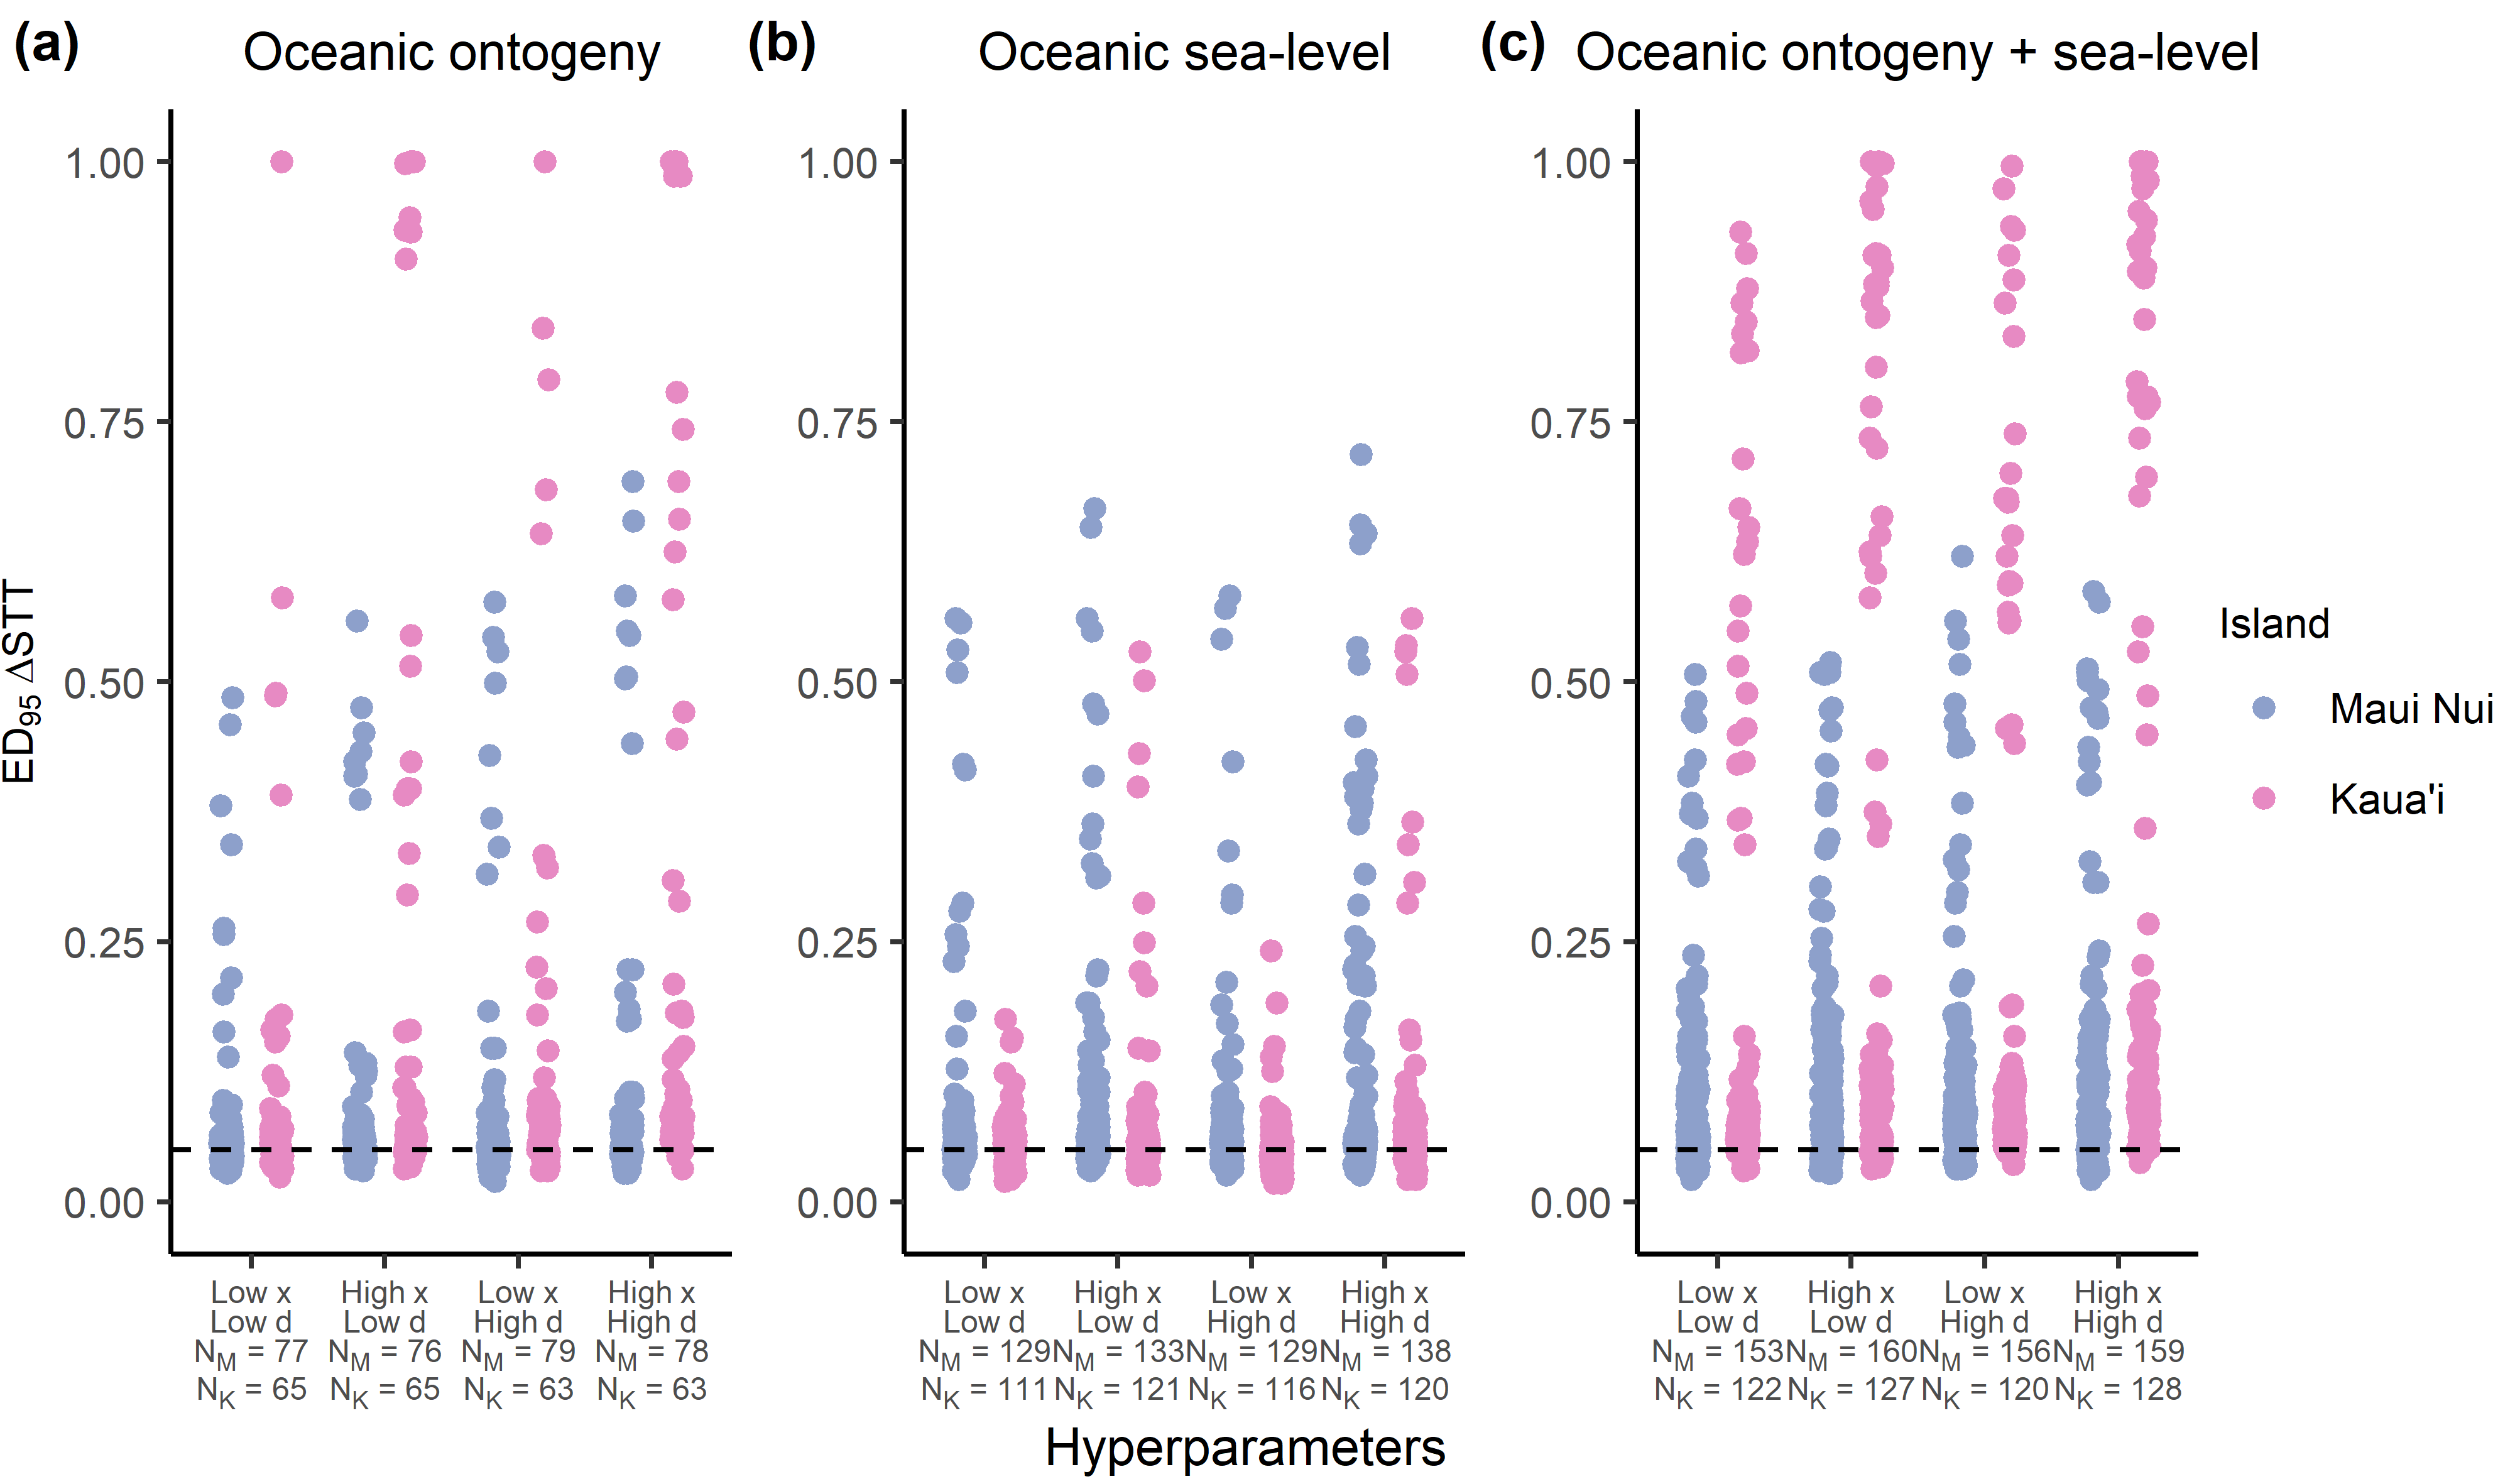
\includegraphics[width=\textwidth]{Hyperparameters_spec_nltt.png}
    \caption{Strip charts showing the distributions of the $ED_{95}$ statistic for $\Delta$STT for each combination of hyperparameters ($d$ and $x$ controlling the effect of area on the rates of cladogenesis and extinction respectively) for the dynamic area oceanic island scenarios. Each point represents the $ED_{95}$ for a single parameter set with the specified hyperparameters on the \textit{x}-axis. All plots have a dashed line at 0.05 which is the null expectation of the $ED_{95}$. (a) $\Delta$STT $ED_{95}$ statistic for oceanic ontogeny. (b) $\Delta$STT $ED_{95}$ statistic for oceanic sea-level. (c) the $\Delta$STT $ED_{95}$ statistic for oceanic ontogeny and sea-level. The sample size for each strip is shown for Maui Nui (N\textsubscript{M}) and Kaua'i (N\textsubscript{K}). See Fig. \ref{tab:oceanic_ontogeny_young}-\ref{tab:oceanic_ontogeny_sea_level_old} for parameter combinations.}
    \label{fig:Hyperparameters_spec_nltt}
\end{figure}

\clearpage

\begin{figure}
    \centering
    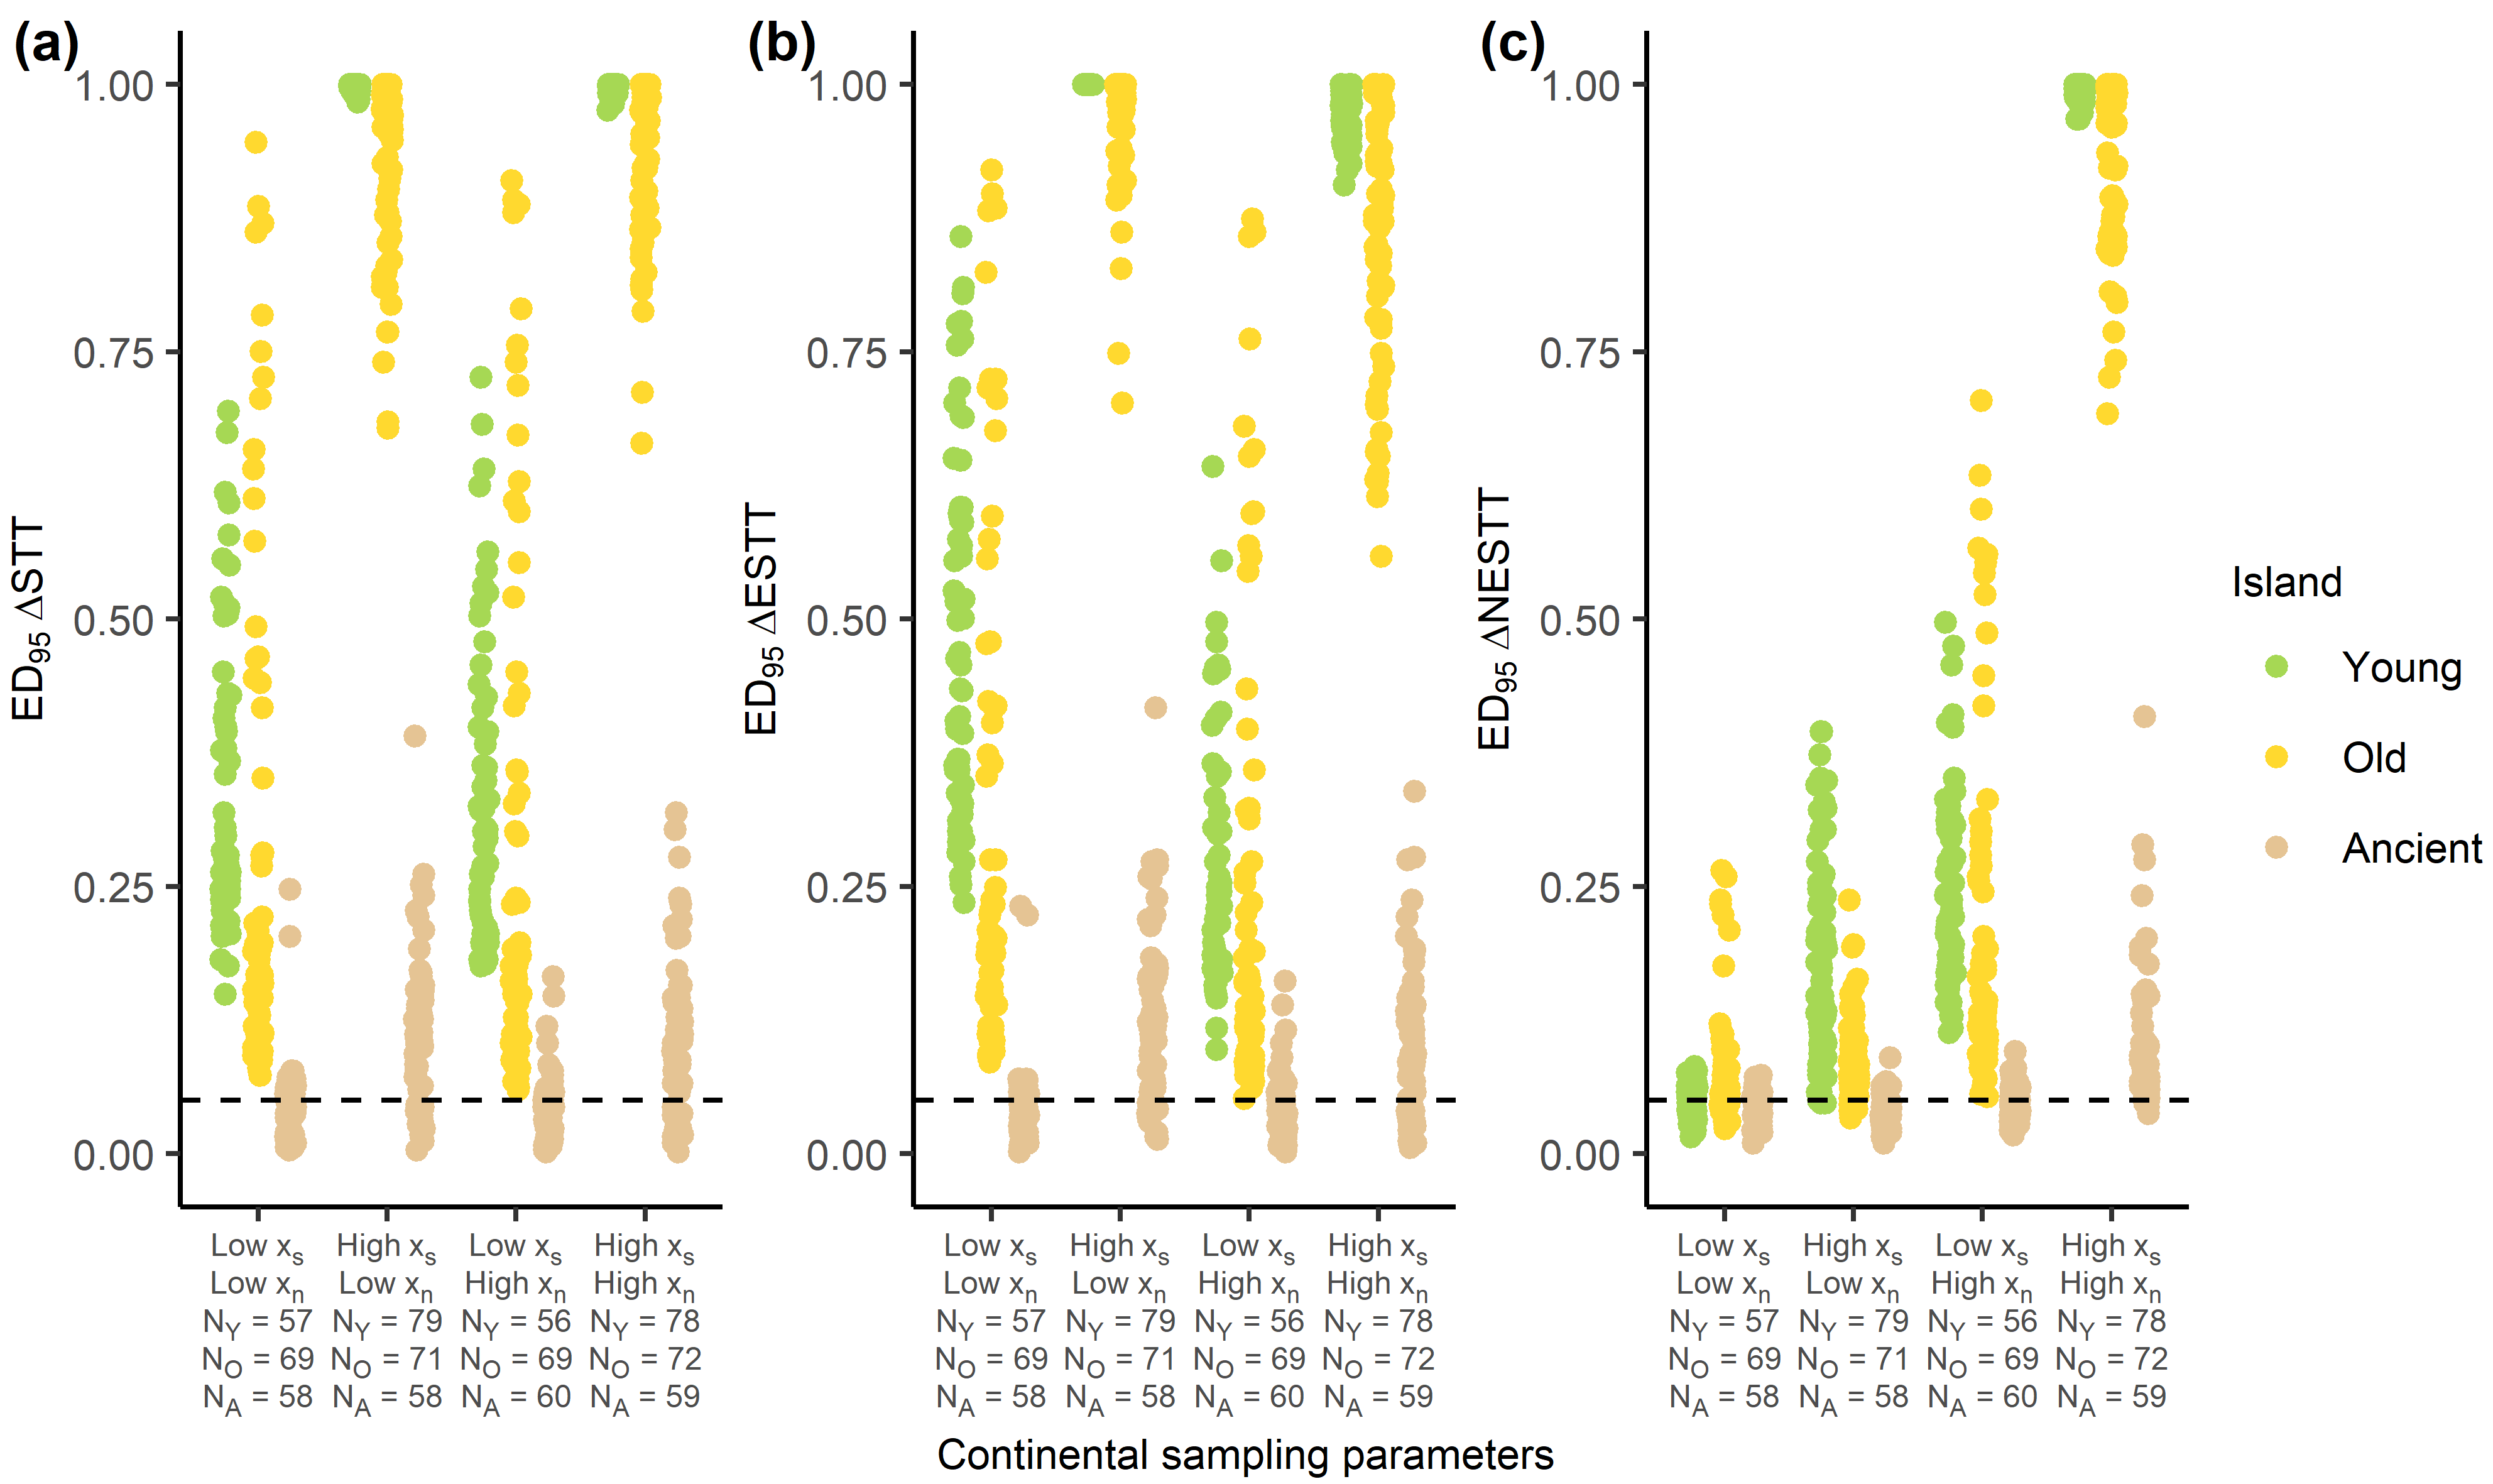
\includegraphics[width=\textwidth]{continental_facet.png}
    \caption{Strip charts showing the distributions of the $ED_{95}$ statistic across the combinations of continental sampling parameters ($x_s$ and $x_n$), for each island age. Each point represents the $ED_{95}$ for a single parameter set with continental sampling parameters on the \textit{x}-axis. All plots have a dashed line at 0.05, which is the null expectation of the $ED_{95}$. Metrics plotted are: (a) $\Delta$STT $ED_{95}$ statistic, (b) $\Delta$ESTT $ED_{95}$ statistic, and (c) $\Delta$NESTT $ED_{95}$ statistic. The sample size for each strip is shown for young islands (N\textsubscript{Y}), old islands (N\textsubscript{O}), and ancient islands (N\textsubscript{A}), sample size for (a), (b) and (c) are the same. See Fig. \ref{tab:continental} for parameter combinations.}
    \label{fig:continental_facet}
\end{figure}

\clearpage

\begin{figure}
    \centering
    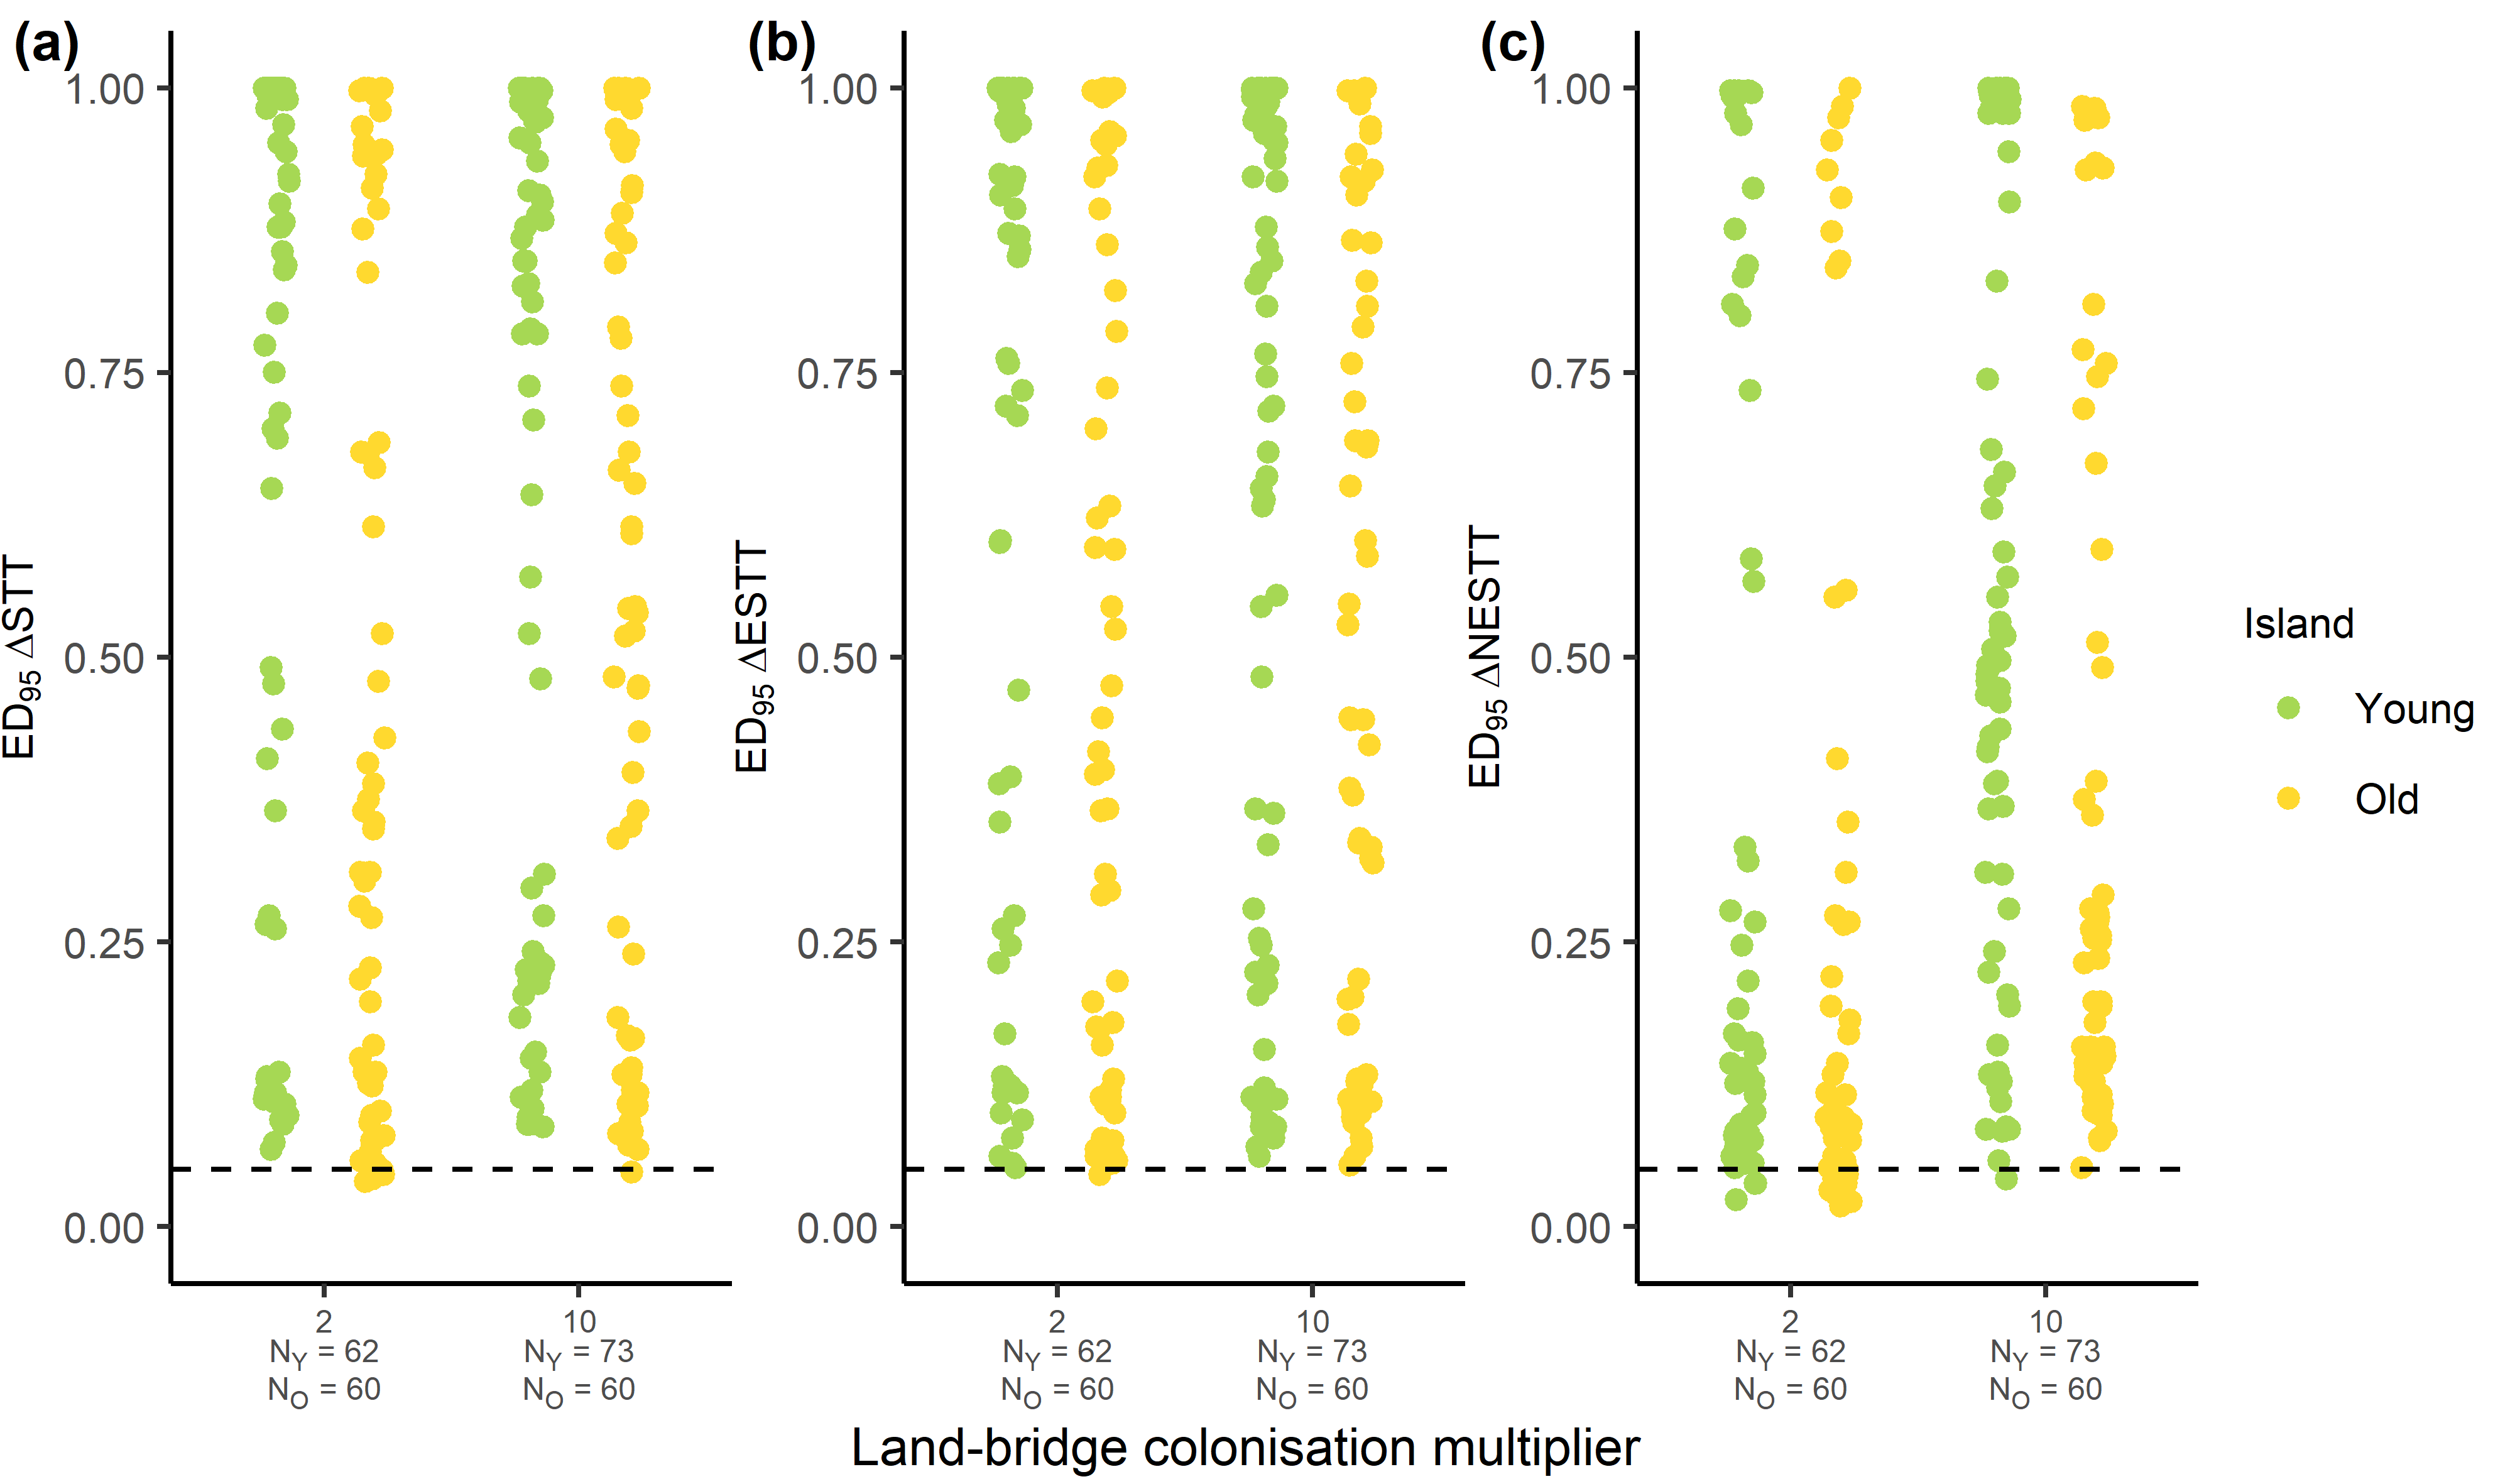
\includegraphics[width=\textwidth]{Land-bridge colonisation multiplier_spec_nltt.png}
    \caption{Strip charts showing the influence of different land-bridge colonisation multipliers (i.e., the factor by which the colonisation rate increases when the land-bridge is present). Each point represents the $ED_{95}$ for a single parameter set. All plots have a dashed line at 0.05 which is the null expectation of the $ED_{95}$. Metrics plotted are: (a) $\Delta$STT $ED_{95}$ statistic, (b) $\Delta$ESTT $ED_{95}$ statistic, and (c) $\Delta$NESTT $ED_{95}$ statistic. The sample size for each strip is shown for young islands (N\textsubscript{Y}) and old islands (N\textsubscript{O}). See Fig. \ref{tab:continental_lb_young}-\ref{tab:continental_lb_old} for parameter combinations.}
    \label{fig:Land-bridge colonisation multiplier_spec_nltt}
\end{figure}

\clearpage

\section*{Discussion}

Our analysis shows that a phylogenetic model of island biogeography that does not account for dynamic island area can accurately reconstruct several metrics of biodiversity through time for islands that form \textit{de novo}, i.e. oceanic islands. Our results thus reveal that oceanic island biodiversity governed by time-dependent rates can be approximated with little error even without knowledge of how rates change through time. This suggests that the study of macroevolutionary community dynamics on islands can make progress with phylogenetic data and produce trustworthy results while reconstructions of paleo-area remain unavailable for most islands. Of course, the field of island biogeography still eagerly awaits more paleogeographic and geological data for islands worldwide, but before these become available, our study suggests that reliable insights can be gained with the existing tools and approximations. \\

However, the same model is usually not robust to the presence of species at island formation, a scenario likely in islands that break away from the continent or are connected to the continent by lowlands that may be flooded during interglacial periods. The age of separation of the island from the mainland is a key indicator for robustness of DAISIE to continental islands – the longer the island has been separated, the higher the robustness of the model.

\subsection*{Robustness to area changes on oceanic islands}

The idea of biodiversity on islands being in disequilibrium has been theorised \citep{whittaker_general_2008, fernandezpalacios_towards_2016} and the impact of sea-level change and ontogeny on island diversity and endemism has previously been shown \citep{lim_true_2017, norder_beyond_2019}. Recent attempts at understanding the macroevolutionary dynamics from phylogenetic data have not considered these geological and sea-level changes when making claims about island community assemblage and diversification \citep{valente_equilibrium_2015, valente_simple_2020}. Here we have shown that although in reality island communities are governed by geological and sea-level dynamics, a simple phylogenetic model of island biogeography can reconstruct diversity dynamics (number of species at present and how they vary through time, as well as the numbers of colonists at present) with little error. The robustness found within this study for oceanic islands may be due to island diversity not declining as fast as expected in nature. The relationship between extinction and island area is inspired by the species-area relationship historically found to be a power law \citep{dengler_which_2009}. \cite{valente_simple_2020} showed that the relationship between island area and extinction was better described by a power law compared to a sigmoidal relationship, but extensions of the power law have not been explored. Other formulations resulting in fewer species at smaller areas could have implications for model robustness \citep{plotkin_predicting_2000}. \\

Traditionally, models that estimate macroevolutionary dynamics from reconstructed phylogenies (i.e. only extant species) can only analyse a single phylogeny, excluding species-poor clades due to insufficient data. By contrast, DAISIE is a phylogenetic model that estimates the macroevolutionary dynamics for an entire community of island species (composed of multiple independent “phylogenies”, many of which with only a single species). This facilitates the investigation of questions that were previously difficult to address on evolutionary time scales in the field of island biogeography, for example whether equilibrium or non-equilibrium dynamics operate on an island \citep{valente_equilibrium_2015}. The precision of the model has been validated when the inference process is matched by the generating process \citep{valente_equilibrium_2015, valente_recent_2017, valente_using_2018}, and in this study the model has been shown to accurately infer and reconstruct island diversity patterns when influenced by area. \\

The minimal error made by DAISIE when inferring parameters from data produced under realistic island ontogeny of two Hawaiian Islands supports the reliability of previous results using the framework. As an example, the Gal\'{a}pagos and Macaronesian archipelagos have complex geographic histories, experiencing rapid island formation from a mantle plume, followed by slow subsidence, and both systems have undergone area changes due to sea-level fluctuations \citep{fernandez-palacios_reconstruction_2011, ali_exploring_2014, geist_2014_paleogeographic, rijsdijk_quantifying_2014}. DAISIE has been applied to the avifauna of the Gal\'{a}pagos and Macaronesia assuming the current archipelago geography back to the system’s origin. The island ontogeny with sea-level changes within this study resembles the histories of such archipelagos, and by extension indicates the reliability of DAISIE’s previous findings on dynamic oceanic systems. The simulations to test geodynamics do not account for the fact that islands within an archipelago may have been connected and disconnected \citep{aguilee_biogeographic_2021}. However, under the assumption that the archipelago operates as a single island – an assumption most valid for volant species e.g. avifauna of the Gal\'{a}pagos \citep{valente_equilibrium_2015} and Macaronesia \citep{valente_equilibrium_2017} – the change in area through time can mimic archipelago dynamics. \\

The development of an inference model of island biogeography that includes changes in area and changes in isolation could be accomplished, with time-variable rates regularly used in phylogenetic models \citep{condamine_assessing_2019}. The problematic aspect is the risk of overfitting a complex model to information-poor data sets, with oceanic islands typically hosting communities between 10 and 50 species for a given taxon of interest (e.g. birds, \cite{valente_simple_2020}), even when they are typically diverse on the continent. The results we find here also suggest that area-dependent rates do not leave a significant signature on phylogenetic data, and as a result, a new inference model incorporating changes in area may not have adequate information to estimate such time-variable dynamics, and may thus erroneously predict such dynamics. \\

One scenario that is shown to produce higher error in inference performance is when the diversity-dependence mechanism differs from the one assumed by the inference model. This occurs when all species on the island compete (IW diversity-dependence), as has been suggested by the GDM of island biogeography \citep{whittaker_general_2008}. Thus, it is not only the geodynamic assumptions of the model, but also the biological interactions assumed by the model that influence its robustness. For empiricists, model selection among different models of diversity-dependence \citep{etienne_limits_2022} hedges against the possibility of spurious results. While the GDM assumes that diversity-dependence operates at the island and not clade level, recent evidence suggests the opposite \citep{etienne_limits_2022}. \\

\subsection*{Vicariant and land-bridge species cause poor performance}

The largest error when reconstructing several aspects of diversity through the island’s history from DAISIE estimates occurs under continental island scenarios. This error was determined by the number of species initially on the island and the time since the island’s formation. The robustness of DAISIE increased as the number of initial species decreased and the time of island separation from the mainland increased. The lower error for longer island history in the continental island case is likely a result of species turnover erasing the signature of vicariant species initially on the island. In these cases, the longer the island exists, the larger the proportion of species that come from colonisation events from the mainland and more of the initial biota go extinct, and the island becomes quasi-oceanic from a biodiversity perspective. Additionally, empirical evidence indicates that heightened extinction from relaxation on continental islands will erase much of the signal of vicariant species over evolutionary time scales, which would produce reconstructed phylogenies resembling oceanic islands \citep{diamond_biogeographic_1972, halley_dynamics_2016}.\\

The lack of robustness of DAISIE to continental islands only applies to the parameter space that was tested within this study, with a conservative estimate of the probability of vicariant species on the island (0.01 and 0.05). Continental islands in nature may exceed this, but there is little information on the number of species that were initially present on a continental fragment or land-bridge island after isolation, as well as what proportion of those species were endemic. DAISIE has been applied to the continental archipelagos of New Zealand \citep{valente_deep_2019} and the Greater Antilles  \citep{valente_recent_2017}. New Zealand is estimated to have been isolated from other landmasses for at least 52 million years \citep{schellart_late_2006}, which is a much longer period of time than the age of most volcanic oceanic islands \citep{valente_simple_2020}. \cite{wallace_island_1880} stated that New Zealand’s biota is akin to that of an oceanic island, an idea that is reflected in our results for ancient continental islands. The Greater Antilles is an archipelago consisting of multiple ancient continental fragments and may have been last connected to continental America by a land-bridge at the Eocene-Oligocene transition (35-33 million years ago, \cite{iturralde_paleogeography_1999}). While there are terrestrial species of vicariant origin in the Greater Antilles \citep{brace_unexpected_2015}, phylogenetic data for bats supports overwater dispersal for all extant and recently extinct taxa \citep{valente_equilibrium_2017}. Therefore, our results suggest that previous DAISIE conclusions on ancient continental fragments are reliable. \\

The theory of species dispersal controlled by geological evolution, and specifically land-bridge formation and disappearance was laid out by \cite{simpson_mammals_1940}. Since then it has become clear that land-bridges facilitate dispersal and alterations in species ranges \citep{wilcox_supersaturated_1978}. In the land-bridge simulations studied here we found that higher colonisation can cause shifts in the island community which cannot be accounted for by the simple inference model. The error made on land-bridge islands exemplifies the need to apply models that account for pairwise shifts in community rates \citep{hauffe_lake_2020}. The failure of DAISIE to robustly estimate rates of macroevolution on land-bridge islands shows clear evidence that oceanic and continental islands leave distinct macroevolutionary signatures in phylogenetic data, and thus different model formulations should be used to study their dynamics. Indeed, phylogeographic and paleo-island biogeography studies have revealed that land-bridge islands have unique colonisation, migration and speciation dynamics that often do not fit classic oceanic-island-centric island biogeography (e.g. \cite{papadopoulou_genomic_2015, hammoud_past_2021}). The land-bridge implementation with different rates of land-bridge colonisation used in this study is consistent with how different taxonomic groups or different land-bridges influence colonisation rates. For example, some land-bridges have facilitated large faunal exchanges \citep{odea_formation_2016}, while others have not caused dispersal between island and the continent, leaving a large proportion of endemics on the island \citep{reuter_role_2021}. The different land-bridge colonisation rates are also compatible with different modes of increased colonisation to an island for a period of time, for example the low colonisation multiplier can represent periods of increasing island colonisation via oceanic currents facilitating rafting \citep{ali_mammalian_2010}, whereas the higher colonisation multiplier may represent a physical land-bridge aiding range movement onto islands. 

\subsection*{Robustness studies in phylogenetics}

Testing the performance of a model of species diversification using reconstructed phylogenies, either by testing model adequacy or the type I error rate and power, has previously been explored \citep{davis_exploring_2013, pennell_model_2015, rabosky_model_2015, etienne_how_2016}. However, these studies assume the inference model is the same as the generating model used to simulate the data. Investigating the behaviour of an inference model when the generating model is different has not been frequently used in models fitted to phylogenetic data (but see \cite{simonet_robustness_2018}). At the same time, the robustness of models of phylogenetic inference has been tested and is well established \citep{huelsenbeck_performance_1995, bilderbeek_quantifying_2021}. Interestingly, these studies have shown that under certain conditions a bias favours simple models over more complex alternatives \citep{yang_how_1997, bruno_topological_1999}. The robustness of the DAISIE inference model to violations in its assumptions highlights the justification for general approximations to describe complex phenomena with a high number of degrees of freedom. Biological systems of interest are highly complex, with heterogeneity between individuals scaling up to macroevolutionary dynamics. Therefore, as in other fields of science, approximations are warranted for a generalised understanding of a system, but should be justified through analysis of a model’s robustness to violations. The generality of the robustness pipeline developed here allows for other studies on the robustness of other models under complex generating processes. Alternative hypotheses for island changes are changing isolation, topographical complexity, or evolution of environmental heterogeneity as new islands undergo succession \citep{massol_island_2017, barajasbarbosa_environmental_2020}.

\section*{Acknowledgments}

We would like to thank Shu Xie, Giovanni Laudanno, Richèl J.C. Bilderbeek, and Pratik Rajan Gupte for their input. We would like to thank the Center for Information Technology of the University of Groningen for their support and for providing access to the Peregrine high performance computing cluster. PSN was funded through a FCT PhD Studentship with reference SFRH/BD/129533/2017, co-funded by the Portuguese Ministério da Ciência, Tecnologia e Ensino Superior and the European Social Fund. JWL was funded through a Study Abroad Studentship by the Leverhulme Trust and was also funded by a NWO VICI grant awarded to RSE. LV was funded by a NWO VIDI grant.

\bibliographystyle{apalike}
\bibliography{references}

\clearpage

\newcommand{\beginsupplement}{%
        \setcounter{table}{0}
        \renewcommand{\thetable}{S\arabic{table}}%
        \setcounter{figure}{0}
        \renewcommand{\thefigure}{S\arabic{figure}}%
     }
     
\beginsupplement
\section*{Supplementary Material}
\subfile{supmat}

\end{document}
